\chapter{Experimental Results}
\todo{Is it even worth putting in RRT performance no one uses vanilla RRTs...}
In this chapter we will review the performance of our various algorithms on different types of worlds. These worlds showcase various scenarios that a motion planner may be presented with. The IOR-RRT variants' results we show for the first two sections use a memory factor of 0. The results shown are averaged over at least 200 trials.
\section{Worlds with Feasible Paths}
The following section is dedicated to worlds that are more common. These are worlds for which there exists a path from a start configuration to a goal configuration without needing to tolerate any collisions. We will look at two such examples: one that is mostly free space, and one that has many obstacles.

\subsection{Simple Minimal Obstacle World}
The first world of this type can be seen in Figure \ref{fig:feasible_world} and algorithm performance can be seen in Table \ref{tab:feasible_world}. 

\begin{figure}[h!]
    \centering
    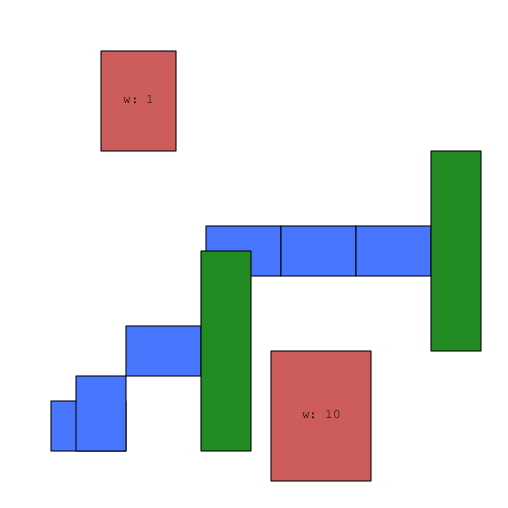
\includegraphics[width=0.5\textwidth]{feasible_world}
    \caption{Common Feasible World}
    \label{fig:feasible_world}
\end{figure}

\begin{table}[h!]
\begin{tabular}{@{}llllll@{}}
\toprule
Algorithm & Success(\%)  & Failure Time  & Success Time  & Path Length & Cover\\ 
\midrule
MCR & 100 & 0.00 & 34.287 & 5460.661 & 2.38 \\
RRT & 19 & 3.95 & 2.48 & 5561.92 & 0.0 \\ 
Bidirectional RRT & 100 & 0.00 & 0.96 & 5432.94 & 0.0 \\
Greedy IOR-RRT & 100 & 0.00 & 0.79 & 5116.33 & 1.4 \\
Probabilistic IOR-RRT & 100 & 0.00 & 0.83 & 5099.30 & 2.8 \\
OIRRT & 100 & 0.00 & 0.54 & 4710.94 & 10.2 \\
Repeated IOR-RRT & 100 & 0.00 & 7.77 & 4653.65 & 0.0 \\
Single Search IOR-RRT & 100 & 0.00 & 1.35 & 5570.78 & 0.1 \\
Repeated Search IOR-RRT & 100 & 0.00 & 1.43 & 5460.72 & 0.0 \\
\bottomrule
\end{tabular}
\caption{Algorithm Performance on Minimal Obstacle World}
\label{tab:feasible_world}
\end{table}

The immediate observation is that despite being largely free space, the normal RRT fails to find paths frequently. Unsurprisingly the algorithms designed to find collision free paths when they exist (bidirectional RRT, Single Search IOR-RRT, Repeated Search IOR-RRT) do find a collision free path on this planning problem. The repeated IOR-RRT has the same performance as measured by the cover, even though it is not designed to find minimal length covers; its success is a result of simply running the same IOR-RRT more times than the normal IOR-RRTs resulting in more opportunities to find a good path. Unsurprisingly, the obstacle ignorant RRT performs poorly in the cover measure but excels in the time measure. The MCR algorithm however fails to find the true 0 cover MCR solution but also takes the most time of any algorithm.

\subsection{Cluttered World With Free Path}
In Figure \ref{fig:many_obstacles_feasible_world} we see a possible situation wherein a feasible path exists, but it is difficult to obtain. Table \ref{tab:many_obstacles_feasible_world} summarizes algorithm performance.

\begin{figure}[h!]
    \centering
    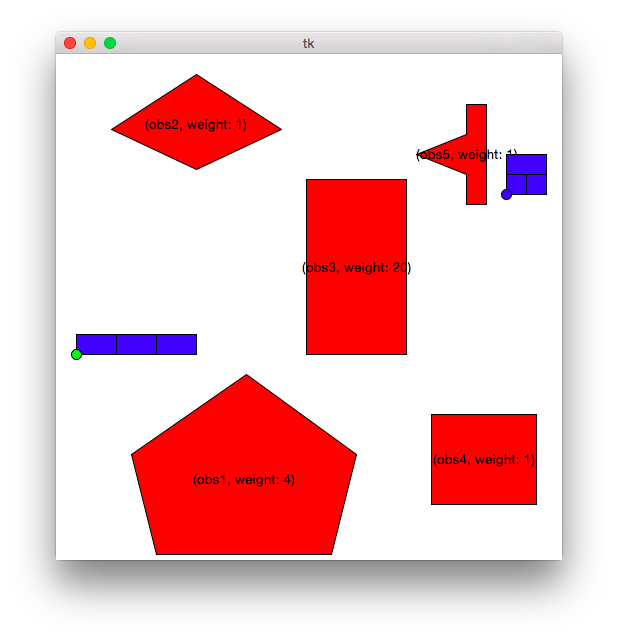
\includegraphics[width=0.5\textwidth]{many_obstacles_feasible_world}
    \caption{Cluttered Feasible World}
    \label{fig:many_obstacles_feasible_world}
\end{figure}


\begin{table}[h!]
\begin{tabular}{@{}llllll@{}}
\toprule
Algorithm & Success(\%)  & Failure Time  & Success Time  & Path Length & Cover\\ 
\midrule
MCR & 100 & 0.00 & 22.55 & 8161.90 & 2.34 \\
RRT & 3 & 2.76 & 2.28 & 7795.35 & 0 \\
Bidirectional RRT & 52 & 9.75 & 4.75 & 8676.26 & 0.00 \\
Greedy IOR-RRT & 100 & 0.00 & 2.94 & 9048.46 & 6.34 \\
Probabilistic IOR-RRT & 100 & 0.00 & 2.53 & 8693.80 & 11.54 \\
OIRRT & 100 & 0.00 & 0.91 & 6477.88 & 22.78 \\
Repeated IOR-RRT & 100 & 0.00 & 25.11 & 8653.24 & 1.28 \\
Single Search IOR-RRT & 100 & 0.00 & 4.29 & 9196.23 & 2.53 \\
Repeated Search IOR-RRT & 100 & 0.00 & 9.68 & 9067.31 & 1.11 \\
\bottomrule
\end{tabular}
\caption{Algorithm Performance on Many Obstacles Feasible World}
\label{tab:many_obstacles_feasible_world}
\end{table}

By introducing a number of narrow hallways between obstacles, the motion planning problem has been made significantly more difficult for traditional motion planning techniques. Bi-RRT success fell to around 50\%. Again, despite the true MCR solution being 0, the bounded time MCR still finds a path with a cover of 2 while taking 22 seconds to solve a single instance of the problem. The two IOR-RRT implementations find paths quickly in under 3s. However, the cover of these two algorithms are high relative to the true MCR score of 0. The greedy removal strategy outperforms the probabilistic removal strategy because of the impact that the induced randomness the sampling strategy adds. Since we use collision counts as measure of the value of a removal, a sampling strategy across this distribution can result in selecting obstacles for removal that are not optimal leading to overall higher cover scores. The repeated probabilistic removal IOR-RRT gets close to the true MCR for the reason described in the previous world experiment in addition to the repeated iterations giving the algorithm the opportunity to select the "right" obstacle to remove. 

\todo{have I mentioned that the search informed IOR-RRTs use greedy removal?}
The search informed RRTs offer interesting insight. The single search informed IOR-RRT only uses a single bidirectional RRT prior to using a greedy IOR-RRT. Since the normal bi-RRT struggles to find paths it follows then that it should performs no better than the multiple search informed IOR-RRT. The cost of searching repeatedly is evident in the runtimeof the repeated search vs single search.


\section{Worlds with Nonexistent Collision Free Paths}
This section will be used to analyze the performance of existing and our proposed algorithms on worlds where no feasible path exists. While these types of worlds will be in the minority of planning problems a motion planner will face it should be robust to these more rare circumstances. 

\subsection{Two Block World}
We start our analysis on unfeasible worlds with a simple analog to the minimal obstacle feasible world example from Figure \ref{fig:feasible_world}. The variant can be seen in Figure \ref{fig:two_soda_world}.

\begin{figure}[h!]
    \centering
    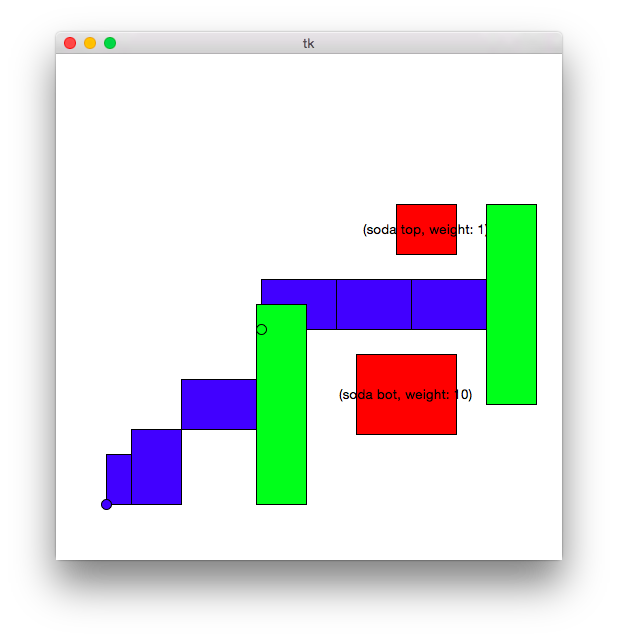
\includegraphics[width=0.5\textwidth]{two_soda_world}
    \caption{Two Box Unfeasible World}
    \label{fig:two_soda_world}
\end{figure}

\begin{table}[h!]
\begin{tabular}{@{}llllll@{}}
\toprule
Algorithm & Success(\%)  & Failure Time  & Success Time  & Path Length & Cover\\ 
\midrule
MCR & 100 & 0.00 & 12.58 & 6060.29 & 1.10 \\
RRT & 0 & 0.83 & 0.00 & 0.00 & 0.00 \\
Bidirectional RRT & 0 & 4.31 & 0.00 & 0.00 & 0.00 \\
Greedy IOR-RRT & 100 & 0.00 & 1.40 & 5151.30 & 2.00 \\
Probabilistic IOR-RRT & 100 & 0.00 & 1.36 & 5076.79 & 2.57 \\
OIRRT & 100 & 0.00 & 0.61 & 4718.62 & 10.94 \\
Repeated IOR-RRT & 100 & 0.00 & 14.06 & 5221.01 & 1.00 \\
Single Search IOR-RRT & 100 & 0.00 & 4.58 & 5314.93 & 1.55 \\
Repeated Search IOR-RRT & 100 & 0.00 & 17.29 & 5295.37 & 1.65 \\
\bottomrule
\end{tabular}
\caption{Algorithm Performance on Two Block Unfeasible World}
\label{tab:two_soda_world}
\end{table}

Naturally because the RRT and Bidirectional RRT search strategies only work in feasible worlds, it is unsurprising that these two algorithms fail in this world. For the other worlds that are unfeasible, we will omit their performance since they necessarily fail. The optimal path cover in this example is a cover of weight one.  We note that in this unfeasible world with only two obstacles, the MCR algorithm takes around 13 seconds before returning a path with a good cover. This has to do with the fundamental MCR algorithm issue of not knowing when to return the found path (since it looks for iteratively better paths than a single path). 

The RRT variant algorithms we propose perform similarly aside from the obstacle ignorant RRT which naturally will find a path that collides with the top and bottom blocks. The general trend is search informed search outperforms any of the individual IOR-RRT options but is outperformed by the repeated IOR-RRT. Additionally there is minimal impact on path lengths from any of these algorithms.




% \subsection{Almost Feasible Path World (MCR shines)}
% \todo{THIS IS GOING TO CHANGE}

% \begin{figure}[h]
%     \centering
%     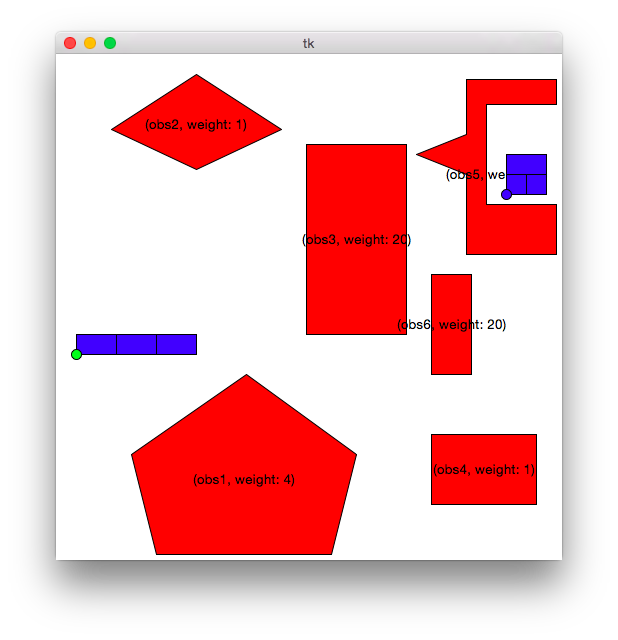
\includegraphics[width=0.5\textwidth]{many_obstacles_unfeasible_world}
%     \caption{Nearly Feasible World}
%     \label{fig:many_obstacles_unfeasible_world}
% \end{figure}

% \begin{table}
% \begin{tabular}{@{}llllll@{}}
% \toprule
% Algorithm & Success(\%)  & Failure Time  & Success Time  & Path Length & Cover\\ 
% \midrule
% MCR & 100 & 0.00 & 51.05 & 9083.23 & 3.44 \\
% RRT & 0 & 2.92 & 0.00 & 0.00 & 0.00 \\
% Bidirectional RRT & 0 & 3.48 & 0.00 & 0.00 & 0.00 \\
% Greedy IOR-RRT & 100 & 0.00 & 1.97 & 7175.5 & 19.75 \\
% Probabilistic IOR-RRT & 100 & 0.00 & 2.40 & 7454.49 & 20.33 \\
% OIRRT & 100 & 0.00 & 1.05 & 6614.65 & 26.52 \\
% Repeated IOR-RRT & 100 & 0.00 & 22.99 & 8620.46 & 8.45 \\
% Single Search IOR-RRT & 100 & 0.00 & 2.57 & 7354.78 & 20.09 \\
% Repeated Search IOR-RRT & 100 & 0.00 & 5.63 & 7346.93 & 18.98 \\
% \bottomrule
% \end{tabular}
% \caption{Algorithm Performance on Many Obstacles Unfeasible World}
% \label{tab:many_obstacles_unfeasible_world}
% \end{table}



\subsection{Cluttered World with Greedy Minimum Cover Path} \label{res:cluttered_world}
Here we will examine the performance of the algorithms on worlds where the best cover paths exist through the direct path from the start to the goal. We would like to understand how the performance of our algorithms changes with the not only the number of obstacles but the location of the best paths.

\begin{figure}[h!]
    \centering
    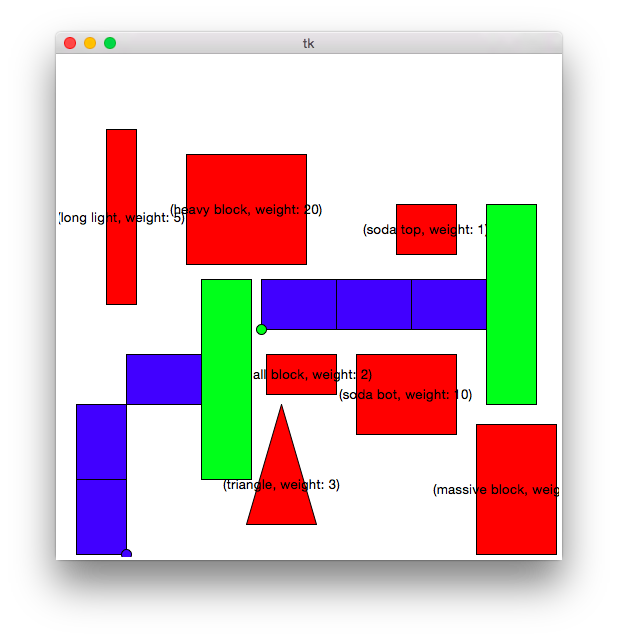
\includegraphics[width=0.5\textwidth]{cluttered_world}
    \caption{Cluttered World With Greedy Path of Minimum Cover}
    \label{fig:cluttered_world}
\end{figure}
\todo{Is it worth showing the 150 iterations greedy fails but probabilistic doesnt?}
With an increased number of RRT iterations we see the behavior in Table \ref{tab:cluttered_world}. 

\begin{table}
\begin{tabular}{@{}llllll@{}}
\toprule
Algorithm & Success(\%)  & Failure Time  & Success Time  & Path Length & Cover\\ 
\midrule
MCR & 100 & 0.00 & 118.69 & 4891.49 & 19.04 \\
Greedy IOR-RRT & 100 & 0.00 & 4.11 & 4656.24 & 16.30 \\
Probabilistic IOR-RRT & 100 & 0.00 & 5.36 & 4927.45 & 20.09 \\
OIRRT & 100 & 0.00 & 1.40 & 5187.00 & 55.08 \\
Repeated IOR-RRT & 100 & 0.00 & 52.81 & 4617.88 & 15.96 \\
Single Search IOR-RRT & 100 & 0.00 & 8.66 & 4603.05 & 16.25 \\
Repeated Search IOR-RRT & 100 & 0.00 & 27.95 & 4576.23 & 16.65 \\
\bottomrule
\end{tabular}
\caption{Algorithm Performance on Cluttered World (With Greedy MCR Path)}
\label{tab:cluttered_world}
\end{table}

Again we see that the MCR algorithm suffers heavily from a longer running time. This high running time is partially a result of the MCR algorithm being one directional. Even if the $k$ frontier is high enough to find $S^*$, it may not succeed at finding the right connections to build the path resulting in a high cover. Since we use a version of MCR where the exit condition is based on the iteration number relative to the best cover found, the number of iterations we must run stays high causing a higher computation time. Additionally because the obstacle weights are widely distributed the algorithm spends a lot of time searching frontiers that cannot yield better path covers. The MCR algorithm's performance is tied to the size of the cover rather than the number of obstacles in the world, which is a problem in worlds with relatively few obstacles but with different weights. Unfortunately this is the more common scenario. Additionally MCR does not find a good path cover either.

The greedy IOR-RRT finds paths with good covers as would be expected from the best path being a greedy path. Since goal biasing encourages growing towards the other tree, it would induce collisions with obstacles in the direct path from the start to the goal. Then the greedy removal strategy would select these obstacles for removal and a good path cover would be found. It is also clear then that the probabilistic removal strategy would lead to on average higher cover paths because it may deviate from the clear greedy path. The search informed algorithms perform the same from a cover perspective as the greedy removal IOR-RRT. Since the space is filled by obstacles, without removing any obstacles there is little space that the search strategy can fill in and accumulate collision information about. The added information is only marginally helpful. Additionally the repeated search informed RRT faces a big penalty in time performance because there does not exist a collision free path; the repeated attempts at looking for collision free paths without gaining additional information incurs no benefits at the expense of time.

\todo{why is some sections double spaced and some single spaced?}


\subsection{Cluttered World with Non-Greedy Minimum Cover Path}
In this last test we use a world that has the same layout as the previous world but with shifted obstacle weights such that the minimum cover path is no longer greedy but follows the top and left edges. 

\begin{figure}[h!]
    \centering
    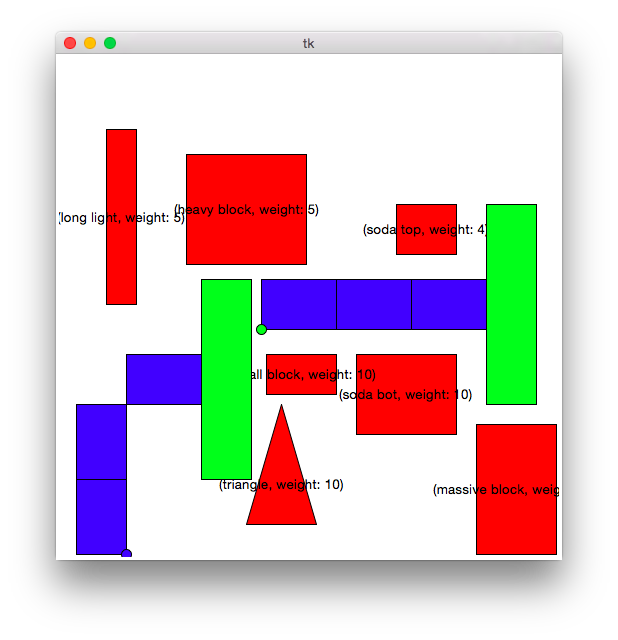
\includegraphics[width=0.5\textwidth]{top_light_cluttered_world}
    \caption{Cluttered World With Non-Greedy Path Of Minimum Cover}
    \label{fig:top_light_cluttered_world}
\end{figure}

\begin{table}[h!]
\begin{tabular}{@{}llllll@{}}
\toprule
Algorithm & Success(\%)  & Failure Time  & Success Time  & Path Length & Cover\\ 
\midrule
MCR & 100 & 0.00 & 163.32 & 6789.82 & 22.43 \\
RRT & 0 & 0.93 & 0.00 & 0.00 & 0.00 \\
Bidirectional RRT & 0 & 4.58 & 0.00 & 0.00 & 0.00 \\
Greedy IOR-RRT & 100 & 0.00 & 4.10 & 5189.46 & 25.15 \\
Probabilistic IOR-RRT & 100 & 0.00 & 5.45 & 5412.72 & 24.28 \\
OIRRT & 100 & 0.00 & 1.34 & 5222.05 & 59.07 \\
Repeated IOR-RRT & 100 & 0.00 & 50.29 & 5860.71 & 14.75 \\
Single Search IOR-RRT & 100 & 0.00 & 9.04 & 5414.53 & 25.13 \\
Repeated Search IOR-RRT & 100 & 0.00 & 27.03 & 5440.75 & 27.00 \\
\bottomrule
\end{tabular}
\caption{Algorithm Performance on Cluttered World (With Non-Greedy MCR Path)}
\label{tab:top_light_cluttered_world}
\end{table}

We see that the greedy removal IOR-RRT is slightly outperformed by the probabilistic removal IOR-RRT. Since the ideal path is no longer along the greedy path from start to goal, the probabilistic removal strategy can succeed at opening up the space that the greedy removal strategy will not. Additionally, for the reasons mentioned in \ref{res:cluttered_world}, the search does not yield any benefit. Repeated IOR-RRT excels in this world due to the repeated chance at finding good paths. 

\section{Discussion on Memory Factor Impact}
This section is dedicated to the impact of the memory factor on the IOR-RRT. Specifically we test the impact using the greedy removal IOR-RRT as the greedy removal strategy generally outperformed the probabilistic removal strategy. We use all memory factors in [0.0, 0.1, 0.3, 0.5, 0.7, 0.9, 1.0].

\begin{table}[h!]
\begin{tabular}{@{}llll@{}}
\toprule
Memory Factor & Two Block World(\%)  & Cluttered Greedy Path  & Cluttered Non-Greedy Path \\ 
\midrule
0.0 & 1.80 & 16.21 & 25.10 \\
0.1 & 1.74 & 16.09 & 25.16 \\
0.3 & 1.54 & 16.34 & 25.50 \\
0.5 & 1.78 & 16.92 & 25.51 \\
0.7 & 1.76 & 17.50 & 25.31 \\
0.9 & 2.00 & 19.51 & 25.35 \\ 
1.0 & 1.96 & 21.08 & 25.07 \\
\bottomrule
\end{tabular}
\caption{Covers Found by Greedy Removal IOR-RRT}
\label{tab:memory_factor_no_impact}
\end{table}

For all memory factors on all the worlds in Table \ref{tab:memory_factor_no_impact}, the greedy removal IOR-RRT had 100\% success rate. Moreover by inspection we see that there is no clear winner in which memory factor leads to the lowest found cover. Specifically the memory factor has negligible impact on the cover of the paths found. 

However, under certain conditions the memory factor can have an impact on the IOR-RRT's ability to find paths. Consider the example world in Figure \ref{fig:memory_factor_world} and the results of using the greedy removal IOR-RRT in Table \ref{tab:memory_factor_impact}.


\begin{figure}[h!]
    \centering
    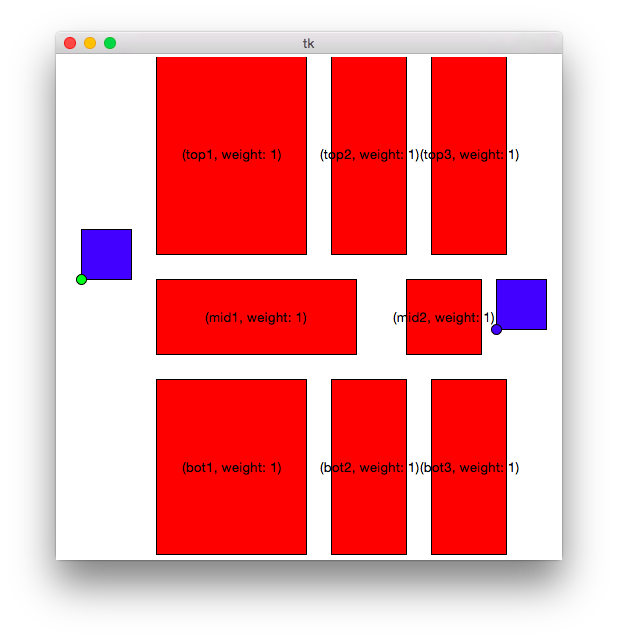
\includegraphics[width=0.5\textwidth]{memory_factor_world}
    \caption{World with Close Clustered Obstacles}
    \label{fig:memory_factor_world}
\end{figure}

\begin{table}[h!]
\begin{tabular}{@{}lllll@{}}
\toprule
Memory Factor & Success Rate(\%)  & Success Time & Path Length & Cover \\ 
\midrule
0.0 & 73.6 & 1.16 & 2223.69 & 2.35 \\
0.1 & 69.6 & 0.98 & 2201.90 & 2.39 \\
0.3 & 61.4 & 0.94 & 2188.36 & 2.27 \\
0.5 & 51.2 & 0.80 & 2153.86 & 2.21 \\
0.7 & 43.4 & 0.69 & 2176.99 & 2.18 \\
0.9 & 28.4 & 0.56 & 2216.65 & 2.17 \\ 
1.0 & 24.4 & 0.40 & 2190.09 & 2.18 \\
\bottomrule
\end{tabular}
\caption{World with Memory Factor Impact}
\label{tab:memory_factor_impact}
\end{table}

We see that low memory factors are correlated with success in finding paths in some situations. Low memory factors lead to higher rates of path discovery because it biases the planner to removing obstacles that are now exposed to collisions in the opened space. With a low removal frequency, collisions are accumulated for a longer period of time. Then, after removing an obstacle and scaling the collision counts by the memory factor, with a high memory factor there may still be a substantial collision count for the other obstacles that were in collision. Consequently the next removal cycle may select one of those original obstacles for removal. Holding the number of removals constant, this can be a wasted obstacle removal. 

In the case of Figure \ref{fig:memory_factor_world}, collisions are many times evenly split among obstacles "mid1" and "top1". This results in, with a high memory factor, both obstacles being removed rather than just one of them. Since there aren't enough removal cycles to remove enough obstacles after removing both of these obstacles, no path is found, leading to the lower success rate. This then motivates using 0 memory factor and restarting our counting of collisions after every removal. Funamentally, this is the right choice as well as we are interested in finding a path from a start configuration to a goal configuration using collision counts as a measure of importance. This suggests that we should always favor exploring new space instead of reducing risk by keeping old memory. This is epecially true when the speed and success at finding a path is more valuable than a more correct path and possibly no path.


